% Scenario: Protecting Passenger Personal and Travel Information
\newcommand{\scenarioOneInformation}{
\begin{table}[H]
    \centering
    \begin{tabularx}{\textwidth}{@{} lX @{}}
    \toprule
    \textbf{Aspect} & \textbf{Details} \\
    \midrule
    Source & Passenger utilizing the TrIP system to manage their travel plans. \\
    Stimulus & The passenger enters personal and travel data into the system. \\
    Artifact & Encrypted Account Lookup Database within the TrIP system. \\
    Response & The system securely stores the passenger's data using state-of-the-art encryption both at rest and in transit, ensuring that personal and travel information is not accessible by unauthorized entities. Access to this data is restricted to specific operations within the TrIP system that require passenger verification. \\
    Measure & Passenger data breaches are non-existent, and passengers report a high level of trust in the system's data protection capabilities. Security logs show no unauthorized access, affirming the integrity of the encryption measures. \\
    \bottomrule
    \end{tabularx}
    \caption{Scenario for Security - Passenger Data Protection}
    \label{table:passenger_data_security}
\end{table}
}

% Scenario: Secure Payment Processing for Passenger Transactions
\newcommand{\scenarioTwoInformation}{
\begin{table}[H]
    \centering
    \begin{tabularx}{\textwidth}{@{} lX @{}}
    \toprule
    \textbf{Aspect} & \textbf{Details} \\
    \midrule
    Source & Passenger making a payment through the TrIP system. \\
    Stimulus & The passenger chooses a payment method and initiates a transaction. \\
    Artifact & Bank interfaced with TrIP system for processing payments. \\
    Response & The bank processes the payment with rigorous security protocols, ensuring that the payment information is handled in a secure, encrypted channel. The system guarantees that payment data is never stored within the TrIP system and is managed exclusively by the bank, providing an additional layer of security. \\
    Measure & Payment transactions are completed with zero incidents of data compromise, and the response time for transaction completion remains within 3 seconds. Post-transaction audits confirm the absence of payment data retention within the TrIP system. \\
    \bottomrule
    \end{tabularx}
    \caption{Scenario for Security - Secure Payment Transactions}
    \label{table:payment_transaction_security}
\end{table}
}

% Scenario: Controlled Access to Passenger Account Data
\newcommand{\scenarioThreeInformation}{
\begin{table}[H]
    \centering
    \begin{tabularx}{\textwidth}{@{} lX @{}}
    \toprule
    \textbf{Aspect} & \textbf{Details} \\
    \midrule
    Source & Passenger subscribing to a specific tycoon's services within the TrIP system. \\
    Stimulus & The subscribed tycoon requests access to the passenger's account data for service personalization. \\
    Artifact & Tycoon API enabling access control to passenger data within the TrIP system. \\
    Response & The TrIP system authenticates the tycoon's request through the Tycoon API, which validates that only the tycoon with whom the passenger is subscribed can retrieve the required data. This ensures that each tycoon can access only their passengers’ data, thus maintaining strict data access control and privacy. \\
    Measure & Regular audits indicate 100\% compliance with data access policies, with no reported incidents of data leakage or unauthorized access. Passenger feedback confirms trust in the data privacy practices of the TrIP system. \\
    \bottomrule
    \end{tabularx}
    \caption{Scenario for Security - Controlled Tycoon Access to Passenger Data}
    \label{table:tycoon_access_control}
\end{table}
}

\section{Information Viewpoint}
We start discussing the Information Viewpoint by analyzing stakeholder concerns that need to be addressed.
We individuated the following user stories:
\begin{itemize}
    \item User stories TODO
\end{itemize}

As a consequence, we decided to prioritize Quality Attributes for this view as indicated in Table~\ref{tab:information_view}.

\begin{table}[h!]
    \centering
    \resizebox{\textwidth}{!}{%
    \begin{tabular}{|l|c|c|c|c|c|c|c|c|c|}
      \hline
      & Usability & Performance & Security & Modifiability & Cost Efficiency & Availability & Safety & Integrability & Maintainability \\
      \hline
      Information View & 
       & % Usability
       & % Performance
      \cellcolor{gray!90}X & % Security (1st priority)
       & % Modifiability
       & % Cost Efficiency
       & % Availability
       & % Safety
       & % Integrability
       \\ % Maintainability
      \hline
    \end{tabular}
    }
    \caption{Information View Prioritized Quality Attributes}
    \label{tab:information_view}
\end{table}

\subsection{View: Main Information View}
\subsubsection{Model}
\begin{figure}[H]
    \centering
    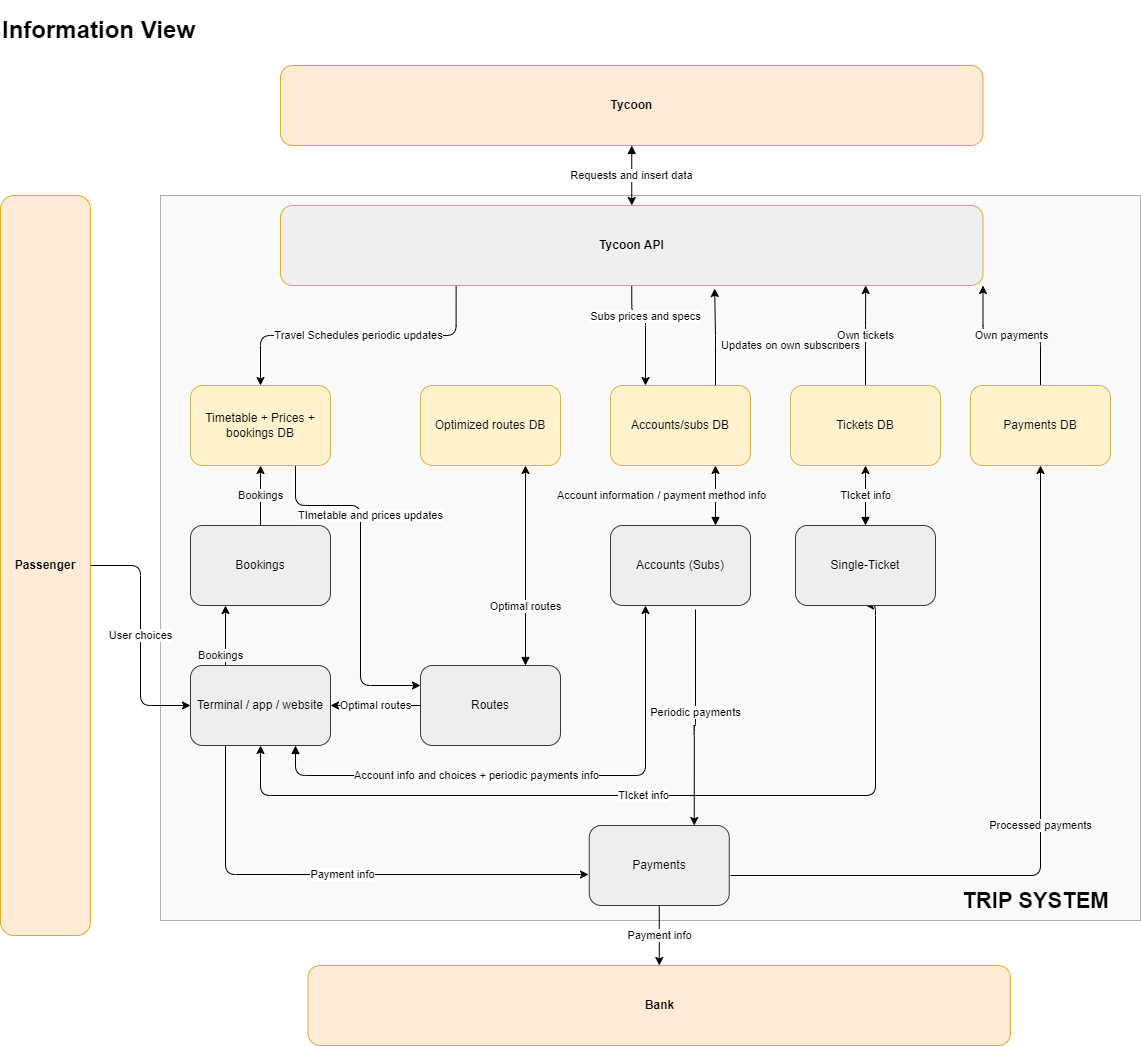
\includegraphics[width=\textwidth]{drawings/views_final_version/information_view.png}
    \caption{Information view.}
    \label{fig:information_view}
\end{figure}

\subsubsection{Description}
The Information View of the TrIP SYSTEM is about how data moves and is stored. The system uses several databases. The Timetable + Prices + Bookings DB keeps track of schedules, prices, and reservations. The Optimized Routes DB has data on the best travel paths. The Accounts/Subs DB holds information on user accounts and subscriptions. The Tickets DB records ticket purchases, and the Payments DB keeps a record of all payments.

Tycoons use the Tycoon API to put in and get data. Passengers use terminals, apps, or websites to book travel and select routes. This choice and payment info go into the databases, updating the system.

The Routes component uses the Optimized Routes DB to give passengers the best travel options. The Accounts (Subs) part handles subscription details and payments, working with the Accounts/Subs DB. For single tickets, there's a separate interface that works with the Tickets DB. Payments process transactions and send completed payment information to the bank.

\subsubsection{Glossary of Elements}

\begin{table}[H]
    \centering
    \caption{Glossary of elements for the Information View of the TrIP SYSTEM.}
    \label{tab:information_view_glossary}
    \begin{tabularx}{\textwidth}{@{}lX@{}} % Use 'X' for auto-adjusting width
    \toprule
    \textbf{Element} & \textbf{Description} \\
    \midrule
    Tycoon & Tycoons responsible for making requests for analysis, and inserting travel data. \\
    Tycoon API & Tycoon's way of interacting to the TrIP system. \\
    Timetable + Prices + bookings DB & Stores data regarding travel schedules, pricing, and booking information. \\
    Optimized routes DB & Contains information on the most efficient travel routes that have been calculated and stored. \\
    Accounts/Subs DB & Maintains records of user accounts and their subscriptions for travel services. \\
    Tickets DB & A database that logs ticket purchases and holds ticket-related information. \\
    Payments DB & Records and processes transactions related to payments within the system. \\
    Passenger & The end-user or customer who utilizes the system for travel services. \\
    Bookings & The system component or interface that passengers interact with to manage and view their bookings. \\
    Terminal / App / Website & The various platforms through which passengers can access the system for services. \\
    Routes & Involves the determination and selection of travel routes within the system. \\
    Accounts (Subs) & Manages the subscription details associated with user accounts. \\
    Single-Ticket & A system or interface that deals with the purchase of individual travel tickets. \\
    Periodic payments & Manages recurring payments, typically for subscription services. \\
    Payments & Processes transactions related to immediate payments within the system. \\
    Processed payments & A log or record of payment transactions that have been completed. \\
    Bank & The financial institution where final payment transactions are processed and funds are transferred. \\
    \bottomrule
    \end{tabularx}
\end{table}

\subsubsection{Analysis on Perspectives}
\textbf{Scenarios}
\scenarioOneInformation
\scenarioTwoInformation
\scenarioThreeInformation

\noindent The Information View of the TrIP system provides a comprehensive architecture designed to handle and safeguard data movement and storage, ensuring the system's integrity and security.

The design segregates data across specialized databases, including those for Timetables + Prices + Bookings, Optimized Routes, Accounts/Subs, Tickets, and Payments. This segregation follows best practices in database security, preventing any single point of compromise and ensuring each database only holds data relevant to its function. Access to these databases is strictly regulated, with the system enforcing robust authentication and authorization mechanisms to verify and control interactions.

Encryption plays an important role in the system, particularly within the Accounts/Subs Database. It protects sensitive passenger information by using encrypted account lookup database. Data at rest within this database, as well as data in transit to and from it, is encrypted, thereby securing personal and travel information from unauthorized access.

Payments are a critical interaction point for the system and its users. The TrIP system approaches this by interfacing directly with banks for payment processing. This interface means that the sensitive financial information is managed within the secure domain of banking institutions, which are inherently designed to handle such data securely. This direct interfacing also implies that the TrIP system does not store payment details, which greatly reduces its liability and exposure to financial data breaches.

The Tycoon API serves as a broker for data access by tycoons. It provides a controlled access point, permitting only authorized tycoons to retrieve passenger data. This access control mechanism is crucial for maintaining passenger privacy and data security. It allows tycoons to access only the data necessary for their service offerings and nothing beyond that.

Using the scenarios provided, we can see how the system's design and technology choices map directly to its operations. Passengers entering their information into terminals or apps can be assured that their data will be encrypted and stored securely, as detailed in the first scenario. Payment processes, as per the second scenario, happen within the secure confines of the banking system. Lastly, the way the Tycoon API manages data requests ensures that passenger data is only accessed by authorized tycoons, enhancing privacy and data protection as outlined in the third scenario.
\subsection{View: Scanning information flows}
\subsubsection{Model}
\begin{figure}[H]
    \centering
    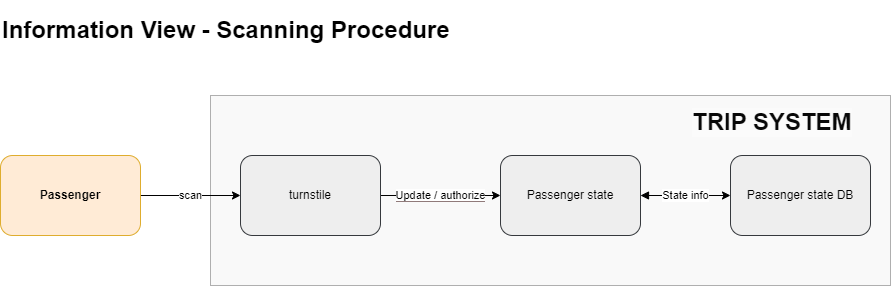
\includegraphics[width=\textwidth]{drawings/views_final_version/information_view scanning.png}
    \caption{Information view related to the scanning procedure.}
    \label{fig:information_view_scanning}
\end{figure}

\subsubsection{Description}
The TrIP SYSTEM's scanning procedure is a sequence that starts with the Passenger, who scans at the Turnstile to gain entry. This triggers the Update/Authorize process, updating the Passenger State with the user's access rights. The Passenger State reflects the user's current permissions within the TRIP SYSTEM. Each user’s information is recorded in the Passenger State DB, a database that tracks and manages user statuses.

\begin{table}[H]
    \centering
    \caption{Legend for the Scanning Procedure in the Information View of the TrIP SYSTEM.}
    \label{tab:scanning_procedure_legend}
    \begin{tabular}{@{}llp{10cm}@{}}
    \toprule
    \textbf{Id} & \textbf{Name} & \textbf{Description} \\
    \midrule
    1 & Passenger & The starting point representing the individual using the TrIP SYSTEM. \\
    2 & Turnstile & The physical or virtual entry point where the passenger scans to gain access. \\
    3 & Update / Authorize & The process that updates the system and authorizes the passenger to proceed. \\
    4 & Passenger State & The current status of the passenger within the system, which is updated after scanning. \\
    5 & Passenger State DB & The database that records the state information of the passenger. \\
    \bottomrule
\end{tabular}
\end{table}

\subsubsection{Analysis on Perspectives}
\textbf{Scenarios}
\scenarioFourInformation


\noindent The information view scanning procedure ensures the passenger data is secure and performant during the scanning proecedure. The TrIP system ensures security by tokenization. By tokenization the TrIP system ensure no sensitive data is stored but only the tokens representing it, which transfers the security risk and the compliance requirements to specialized companies. Also, by recording the user state the system ensures a quick scanning process.
